\question[6]以下物理量为矢量,且单位是国际单位制基本单位的是\key{}
\fourchoices{电流、A}{位移、m}{功、J}{磁感应强度、T}
\begin{solution}{4cm}

\end{solution}



\question[6]如图所示,一对父子瓣手腕,父亲让儿子获胜.若父亲对儿子的力记为$F_1$,儿子对父亲的力记为$F_2$,则\key{}\begin{center}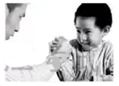
\includegraphics[]{img/image1.png}\end{center}
\fourchoices{$F_1>F_2$}{$F_1$和$F_2$大小相等}{$F_1$先于$F_2$产生}{$F_1$后于$F_2$产生}
\begin{solution}{4cm}

\end{solution}



\question[6]如图所示,新中国成立70周年阅兵仪式上,国产武装直升机排列并保持$"70"$字样编队从天安门上空整齐飞过.甲、乙分别是编队中的两架直升机,则\key{}\begin{center}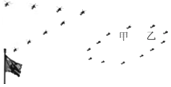
\includegraphics[]{img/image2.png}\end{center}
\fourchoices{以甲为参考系,乙是运动的}{以乙为参考系,甲是运动的}{以甲为参考系,坐在观众席上的观众都是静止的}{以乙为参考系,$"70"$字样编队中所有直升机都是静止的}
\begin{solution}{4cm}

\end{solution}



\question[6]下列说法正确的是\key{}
\fourchoices{α射线的穿透能力比γ射线强}{天然放射现象说明原子具有复杂的结构}{核聚变中平均每个核子放出的能量比裂变中平均每个核子的小}{半衰期跟放射性元素以单质或化合物形式存在无关}
\begin{solution}{4cm}

\end{solution}



\question[6]如图所示,钢球从斜槽轨道末端以$v_0$的水平速度飞出,经过时间t落在斜靠的挡板AB中点.若钢球以$2v_0$的速度水平飞出,则\key{}\begin{center}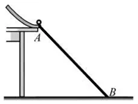
\includegraphics[]{img/image3.png}\end{center}
\fourchoices{下落时间仍为t}{下落时间为2t}{下落时间为$\sqrt{2}t$}{落在挡板底端B点}
\begin{solution}{4cm}

\end{solution}



\question[6]小明在一根细橡胶管中灌满食盐水,两端用粗铜丝塞住管口,形成一段封闭的盐水柱.他将此盐水柱接到电源两端,电源电动势和内阻恒定.握住盐水柱两端将它水平均匀拉伸到原长的$1.2$倍,若忽略温度对电阻率的影响,则此盐水柱\key{}
\fourchoices{通过的电流增大}{两端的电压增大}{阻值增大为原来的$1.2$倍}{电功率增大为原来的$1.44$倍}
\begin{solution}{4cm}

\end{solution}



\question[6]如图所示,电子以某一初速度沿两块平行板的中线方向射人偏转电场中,已知极板长度l,间距d,电子质量m,电荷量e.若电子恰好从极板边缘射出电场,由以上条件可以求出的是\key{}\begin{center}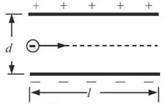
\includegraphics[]{img/image4.png}\end{center}
\fourchoices{偏转电压}{偏转的角度}{射出电场速度}{电场中运动的时间}
\begin{solution}{4cm}

\end{solution}



\question[6]如图所示,单刀双挪开关S先打到a端让电容器充满电$.t=0$时开关S打到b端,$t=0.02s$时LC回路中电容器下极板带正电荷且电荷量第一次达到最大值.则\key{}\begin{center}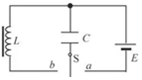
\includegraphics[]{img/image5.png}\end{center}
\fourchoices{LC回路的周期为$0.02s$}{LC回路的电流最大时电容器中电场能最大}{$t=1.01s$时线圈中磁场能最大}{$t=1.01s$时回路中电流沿顺时针方向}
\begin{solution}{4cm}

\end{solution}



\question[6]如图所示,卫星a、b、c沿圆形轨道绕地球运行.a是极地轨道卫星,在地球两极上空约$1000km$处运行;b是低轨道卫星,距地球表面高度与a相等;c是地球同步卫星,则\key{}\begin{center}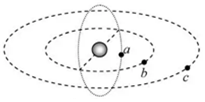
\includegraphics[]{img/image6.png}\end{center}
\fourchoices{a、b的周期比c大}{a、b的向心力一定相等}{a、b的速度大小相等}{a、b的向心加速度比c小}
\begin{solution}{4cm}

\end{solution}



\question[6].如图所示,甲乙两图中的理想变压器以不同的方式接在高压电路中.甲图中变压器原副线圈的匝数比为$k_1$,电压表读数为U,乙图中变压器原副线圈的匝数比为$k_2$,电流表读数为I.则甲图中高压线电压和乙图中高压线电流分别为\key{}\begin{center}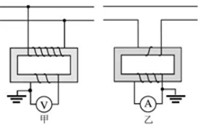
\includegraphics[]{img/image7.png}\end{center}
\fourchoices{$k_1U$,$k_2I$}{$k_{1}U$,$\frac{I}{k_{2}}$}{$\frac{U}{k_{1}}$,$k_2I$}{$\frac{U}{k_{1}}$,$\frac{I}{k_{2}}$}
\begin{solution}{4cm}

\end{solution}



\question[6].如图所示,在光滑绝缘水平面上,两条固定的相互垂直彼此绝缘的导线通以大小相同的电流I.在角平分线上,对称放置四个相同的正方形金属框.当电流在相同时间间隔内增加相同量,则\key{}\begin{center}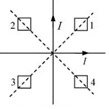
\includegraphics[]{img/image8.png}\end{center}
\fourchoices{1、3线圈静止不动,2、4线圈沿着对角线向内运动}{1、3线圈静止不动,2、4线圈沿着对角线向外运动}{2、4线圈静止不动,1、3线圈沿着对角线向内运动}{2、4线圈静止不动,1、3线圈沿着对角线向外运动}
\begin{solution}{4cm}

\end{solution}



\question[6].如图所示,一束光与某材料表面成$45^°$角入射,每次反射的光能量为入射光能量的k倍($0<k<1$).若这束光最终进入材料的能量为入射光能量的($1-k^2$)倍,则该材料折射率至少为\key{}\begin{center}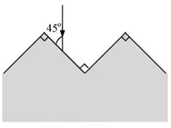
\includegraphics[]{img/image9.png}\end{center}
\fourchoices{$\frac{\sqrt{6}}{2}$}{$\sqrt{2}$}{$1.5$}{2}
\begin{solution}{4cm}

\end{solution}



\question[6].如图所示,在倾角为α的光滑绝缘斜面上固定一个挡板,在挡板上连接一根劲度系数为$k_0$的绝缘轻质弹簧,弹簧另一端与A球连接.A、B、C三小球的质量均为M,$q_A=q_0>0$,$q_B=-q_0$,当系统处于静止状态时,三小球等间距排列.已知静电力常量为k,则\key{}\begin{center}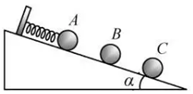
\includegraphics[]{img/image10.png}\end{center}
\fourchoices{$q_{c}=\frac{4}{7}q_{0}$}{弹簧伸长量为$\frac{Mg\sin\alpha}{k_{0}}$}{A球受到的库仑力大小为$2Mg$}{相邻两小球间距为$q_{0}\sqrt{\frac{3k}{7Mg}}$}
\begin{solution}{4cm}

\end{solution}



\question[6].由玻尔原子模型求得氢原子能级如图所示,已知可见光的光子能量在$1.62eV$到$3.11eV$之间,则\key{}\begin{center}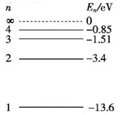
\includegraphics[]{img/image11.png}\end{center}
\fourchoices{氢原子从高能级向低能级跃迁时可能辐射出γ射线}{氢原子从$n=3$的能级向$n=2$的能级跃迁时会辐射出红外线}{处于$n=3$能级的氢原子可以吸收任意频率的紫外线并发生电离}{大量氢原子从$n=4$能级向低能级跃迁时可辐射出2种频率的可见光}
\begin{solution}{4cm}

\end{solution}



\question[6].如图所示,波长为$λ_a$和$λ_b$的两种单色光射入三棱镜,经折射后射出两束单色光a和b,则这两束光\key{}\begin{center}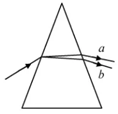
\includegraphics[]{img/image12.png}\end{center}
\fourchoices{照射同一种金属均有光电子逸出,光电子最大初动能$E_Ka>E_Kb$}{射向同一双缝干涉装置,其干涉条纹间距$△x_a>△x_b$}{C.在水中的传播速度$v_a<v_b$}{光子动量$p_a<p_b$}
\begin{solution}{4cm}

\end{solution}



\question[6].如图所示,波源O垂直于纸面做简谐运动,所激发的横波在均匀介质中向四周传播,图中虚线表示两个波面$.t=0$时,离O点5m的A点开始振动$;t=1s$时,离O点$10m$的B点也开始振动,此时A点第五次回到平衡位置,则\key{}\begin{center}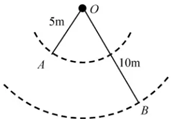
\includegraphics[]{img/image13.png}\end{center}
\fourchoices{波的周期为$0.4s$}{波的波长为2m}{波速为$55\sqrt{3}m/s$}{$t=1s$时AB连线上有4个点处于最大位移}
\begin{solution}{4cm}

\end{solution}



